% Journal of Intelligent Information Systems (Springer) submission.
% Springer Nature template v3.1 (Dec 2024), sn-basic reference style as the journal asks.
% Build: tectonic -X compile main.tex   (or pdflatex, bibtex, pdflatex x2)
% Anonymised for review: no author names, affiliations or repository URL. Restore them for the
% camera-ready version (the author block is in the earlier ICCIDS draft, in git history).
\documentclass[pdflatex,sn-basic,lineno]{sn-jnl}

\usepackage{graphicx}
\usepackage{amsmath,amssymb}
\usepackage{amsthm}
\usepackage{booktabs}
\usepackage{tabularx}
\usepackage{tikz}
\usepackage{pgfplots}
\pgfplotsset{compat=1.17}
\usepackage{url}
\usepackage{algorithm}
\usepackage{algpseudocode}
\algrenewcommand\algorithmicrequire{\textbf{Input:}}
\algrenewcommand\algorithmicensure{\textbf{Output:}}

\theoremstyle{thmstylethree}
\newtheorem{definition}{Definition}
\theoremstyle{thmstyleone}
\newtheorem{proposition}{Proposition}

\newcommand{\rel}[1]{\textsc{#1}}

\hypersetup{hypertexnames=false}
\raggedbottom

\begin{document}

\title[Evidence-Grounded Causal Knowledge Graphs from GDELT]{From GDELT to Causal Knowledge
Graphs: An Evidence-Grounded Algorithm for Building and Querying Causal Chains of Protest Events}

\author{\fnm{Anonymous} \sur{Author(s)}}
\affil{\orgname{Withheld for double-anonymous review}}

\abstract{Event databases such as GDELT record what happened in the news, but not why. We
first show that causes cannot be recovered from GDELT metadata: on 2024 Indian protest events, a
scorer fusing six metadata channels retained shuffled event pairs as often as genuine ones, and
none of the 322 candidates it proposed was a cause supported by the source text. We then present
an algorithm that turns the articles behind GDELT records into a queryable causal knowledge graph.
It extracts events and grievances as verbatim spans, merges reports of the same event across
articles under cannot-link constraints, proposes candidate causes, and accepts a link only when
the article states it, storing the exact supporting quotation. An independent second annotation,
mixed one-to-one with decoys, gates every unreviewed link, and cycles are removed by adjudicating
the quotations on each cycle. A query algorithm answers ``why did this happen?'' and ``what did it
lead to?'' with ranked cause chains in which every step is quoted and sourced, and refuses
questions about places, names or years the graph does not contain. The annotator is pluggable; we used
language model agents. On 2{,}000 articles the algorithm built 1{,}416 sourced causal
links explaining 358 of 373 protests, while human verdicts per published link fell from 1.18 to
0.07. A random audit of 100 unreviewed links found 89 of 99 correct (95\% CI 82--94\%), including
all 69 supported by explicit causal wording; every error rested on implied evidence, most often
between two stages of one campaign.}

\keywords{causal knowledge graphs, event data, GDELT, evidence grounding, LLM-based annotation,
causal question answering}

\maketitle

%% ---------------------------------------------------------------------------------------------
\section{Introduction}\label{sec:intro}

Event databases such as GDELT \citep{gdelt}, ICEWS \citep{icews} and ACLED \citep{acled} convert
news reports into structured records, and analysts routinely put causal questions to them: why did
farmers march on Delhi in February 2024, and what followed the killing of a trainee doctor in
Kolkata in August 2024? The records cannot answer such questions. They hold actors, CAMEO event
codes \citep{cameo}, places and dates, so any causal claim derived from them rests on
co-occurrence, and machine-coded event data are already noisy at that level \citep{hammond}. The
articles behind the records are different: they frequently \emph{state} a cause, in phrases such
as ``protesting against'', ``in response to'' or ``after their march was stopped''.

Research on temporal knowledge graphs (TKGs) has largely optimised link-prediction and forecasting
metrics over such records. A recent survey of causal reasoning over TKGs \citep{survey} argued
that the field rewards temporal association rather than causal validity, and that verifiable
evidence grounding is the missing ingredient. This article puts that argument into practice. It
describes, and evaluates at scale, an algorithm that starts from GDELT and ends with a causal
knowledge graph \citep{hogan} in which every link carries the sentence that supports it, its
source URL and its dates, so that any answer the graph gives can be traced to the text.

Building such a graph by hand does not scale, and delegating annotation to a language model raises
an obvious question: how far can its unreviewed output be trusted? We therefore treat the
annotator as replaceable and fallible, constrain what it can assert, and measure where it fails.
The study is organised around four research questions.

\begin{description}
\item[RQ1] Can causal links between protest events be inferred from GDELT event metadata alone?
\item[RQ2] Can an independent second annotation, calibrated with decoys, replace per-link human
review as the acceptance gate for annotated causal links?
\item[RQ3] How accurate are the causal links that no person reviewed, and where do they fail?
\item[RQ4] Can the resulting graph answer causal questions with traceable chains, and how much
human effort does construction require?
\end{description}

The contributions are as follows.
\begin{enumerate}
\item A negative result (RQ1): a six-channel metadata scorer over GDELT cannot distinguish genuine
cause--effect pairs from shuffled ones, and none of its candidates is supported by the source text.
\item An algorithm that builds an evidence-grounded causal graph from GDELT-linked articles, with
verbatim extraction, cross-article canonicalisation under cannot-link constraints,
quotation-backed causal linking, recovery of stated but unextracted causes, a decoy-calibrated
second-annotation gate and cycle adjudication, at an annotation cost linear in the number of
targets (Section~\ref{sec:method}).
\item A query algorithm that answers causal questions from graph records alone, with ranked quoted
chains, explicit refusal of questions the graph cannot ground, and a report of what was never
searched (Section~\ref{sec:query}).
\item An evaluation on 2{,}000 articles covering gate calibration, graph quality, a component
ablation, a random audit with an error taxonomy, case studies and human effort
(Section~\ref{sec:results}).
\end{enumerate}

Section~\ref{sec:related} reviews related work, Section~\ref{sec:problem} formalises the problem,
Section~\ref{sec:method} presents the construction algorithm and Section~\ref{sec:query} the query
algorithm. Section~\ref{sec:setup} describes the experimental setup, Section~\ref{sec:results}
reports results, Section~\ref{sec:discussion} discusses threats to validity, and
Section~\ref{sec:conclusion} concludes.

%% ---------------------------------------------------------------------------------------------
\section{Related work}\label{sec:related}

\subsection{Event databases and event knowledge graphs}
GDELT codes events from global news with the CAMEO ontology \citep{gdelt,cameo}; ICEWS offers a
curated alternative \citep{icews}, and ACLED codes political violence and protest by hand
\citep{acled}. \citet{hammond} show that machine-coded records are unreliable
at the micro level, through duplication and geolocation error, which is the level at which causal
questions about individual protests are asked. EventKG \citep{eventkg} integrates event-centric
knowledge across sources with temporal relations, and recent work queries GDELT through knowledge
graphs and language models \citep{myers}. None of these resources records why an event happened:
relations between events, where present, are temporal, spatial or participatory, not causal.

\subsection{Reasoning over temporal knowledge graphs}
TKG research has concentrated on completion and forecasting, through time-aware embeddings
\citep{jiang16,garcia18,lacroix20}, recurrent and point-process models
\citep{knowevolve,dyrep,renet,tgn} and rule-based or path-based explanations \citep{tlogic,xerte}.
Validity periods of facts have been derived directly \citep{leblay}, and temporal question
answering has its own benchmarks \citep{cronkgqa,jia21,multitq}. More recent models identify
causal sub-histories for extrapolation \citep{csi} or model how the confidence of a rule decays
over time \citep{huang24}. As the survey cited above observed \citep{survey}, these methods
optimise ranking metrics over associations; none returns a cause that a reader can verify in a
source text. Our query algorithm, by contrast, performs no inference beyond the stored links: its
explanations are paths whose every edge is a quoted statement.

\subsection{Causal relations in text}
Annotated resources for causal language include the Penn Discourse Treebank \citep{pdtb},
SemEval-2010 Task~8 \citep{semeval}, Causal-TimeBank \citep{mirza}, BECauSE \citep{because},
EventStoryLine \citep{storyline} and MAVEN-ERE \citep{mavenere}; \citet{yangsurvey}
survey pattern-based, statistical and neural extractors. These resources annotate causal relations
within a sentence or document. Event-graph methods support explainable causal reasoning
\citep{excar}, and CauseNet \citep{causenet} mines a web-scale graph of causal relations between
concepts, retaining the sentences they were extracted from. News streams have been used to predict
events \citep{radinsky} and to identify predictive causal factors \citep{balashankar}, and
time-series methods recover causal graphs from news-derived signals \citep{maisonnave,runge}. In
the terms of \citet{pearl}, the time-series methods estimate association from observational
signals; the extraction resources stay within one document. We link canonical, dated events and
conditions \emph{across} articles into multi-level chains, and ground each link in a quotation.

\subsection{Language models as annotators and judges}
Language models can annotate text at or above crowd-worker quality \citep{gilardi,tornberg}, stand
in for human evaluation \citep{chiang} and act as autonomous agents \citep{agentsurvey,react}. As
evaluators, however, they show position and self-preference biases \citep{zheng,wangfair}; their
causal reasoning is uneven \citep{kiciman,cladder}; and they can produce fluent but unsupported
output \citep{hallucination}, for which grounding in structured knowledge is one remedy
\citep{pan24}. These findings motivate three design choices: every value an annotation asserts must
occur verbatim in the source; acceptance requires a second annotation made blind to the first; and
the second annotator's discrimination is measured on decoys rather than assumed.

\subsection{Constrained merging and cycle repair}
Merging reports of the same event is a clustering problem with background knowledge: some pairs
must never be joined. Cannot-link constraints were introduced for constrained $k$-means
\citep{wagstaff}; we apply them to union--find merging, where a human-accepted causal link between
two nodes forbids their union. A causal graph must also be acyclic. Strongly connected components,
found with Tarjan's algorithm \citep{tarjan}, locate every cycle; rather than removing the weakest
edge, we remove the edge whose quotation fails to support it, since a confidence-based rule removed
correct links in testing.

\subsection{Positioning}
Table~\ref{tab:compare} contrasts the resulting graph with the resources above along the properties
that matter for causal questions about specific events.

\begin{table}[!htbp]
\caption{Comparison with related resources. ``Quoted support'' means each causal link stores the
text that states it; ``cross-document'' means a link may join events reported in different
articles.}
\label{tab:compare}
\footnotesize
\begin{tabularx}{\textwidth}{@{}Xccccc@{}}
\toprule
Resource & Unit & Causal links & Quoted support & Cross-document & Dated \\
\midrule
GDELT, ICEWS, ACLED \citep{gdelt,icews,acled} & event record & no & -- & -- & yes \\
EventKG \citep{eventkg} & event & no & -- & yes & yes \\
TKG forecasting models \citep{renet,tlogic,csi} & fact quadruple & associative & no & yes & yes \\
EventStoryLine, MAVEN-ERE \citep{storyline,mavenere} & event mention & yes & sentence & no & partly \\
CauseNet \citep{causenet} & concept & yes & yes & yes & no \\
This work & event or condition & yes & yes & yes & yes \\
\bottomrule
\end{tabularx}
\end{table}

%% ---------------------------------------------------------------------------------------------
\section{Problem formulation}\label{sec:problem}

\begin{definition}[Causal evidence graph]
A causal evidence graph is a directed graph $G=(V,E)$. Each node $v\in V$ is either an
\emph{event}, an action with actors, targets, a place and a time range $[\tau^-_v,\tau^+_v]$, or a
\emph{condition}, a standing state or grievance (for example, a policy in force or unpaid dues)
with a validity window. Each edge $e=(u\rightarrow v)\in E$ asserts that $u$ led to $v$ and carries
a relation $r_e\in\mathcal{R}$, a strength $s_e\in\{1,2,3\}$, an evidence type
$q_e\in\{\textit{explicit},\textit{implicit}\}$, a non-empty set of quotations $Q_e$ with their
source URLs, and the claims that support it.
\end{definition}

The relation set $\mathcal{R}$ has five members, \rel{triggers}, \rel{motivates},
\rel{mobilizes}, \rel{escalates} and \rel{prompts\_response}, defined in
Table~\ref{tab:rubric}.

\begin{definition}[Verbatim span]
Let $d$ be an article and $\sigma$ one of its sentences. A string $x$ is a verbatim span of
$\sigma$ if $\sigma[i{:}j]=x$ for some offsets $i<j$. Every field of an extracted node (action,
actors, targets, place, time expression) and every quotation in $Q_e$ must be a verbatim span of
a sentence of a source article; values that fail the check are discarded, never repaired.
\end{definition}

\begin{definition}[Claim and annotations]
A \emph{claim} $c=(u\rightarrow t)$ is one candidate cause $u$ proposed for a target $t$. An
annotator $J$ applies a written rubric to a claim and returns \textit{accept}, with a relation,
strength, evidence type and quotation, or \textit{reject}, with one of eight reason codes. Let
$H(c)$ be a human verdict when one exists (including verdicts carried over from earlier runs),
$A(c)$ the first annotation and $B(c)$ an independent second annotation made without access to
$A(c)$ or its quotation. We write $\bot$ for an absent verdict.
\end{definition}

\begin{definition}[Gate]
A claim $c$ supports an edge if and only if
\begin{equation}
\textsc{PassGate}(c) \;\equiv\; H(c)=\textit{accept} \;\lor\; \bigl(H(c)=\bot \land
A(c)=\textit{accept} \land B(c)\neq\textit{reject}\bigr).
\label{eq:gate}
\end{equation}
\end{definition}

A human verdict therefore always outranks the annotator, and an unreviewed claim needs two
independent acceptances (or an acceptance and an abstention).

\begin{definition}[Causal order and search status]
A claim $(u\rightarrow t)$ is admissible only if $\tau^-_u\le\tau^+_t$, that is, $u$ is not dated
after its effect. Each node reached during expansion records one of three statuses: causes found,
searched with no cause found, or never searched. The absence of a cause and the absence of a search
therefore remain distinct.
\end{definition}

The task is: given GDELT event records $R$, construct $G$ such that (i) every edge has at least one
claim satisfying Eq.~(\ref{eq:gate}); (ii) every quotation is a verbatim span of its source;
(iii) $G$ is acyclic; (iv) no two nodes joined by a human-accepted edge are merged; and (v) the
construction is deterministic, so that the same inputs yield a byte-identical graph. Given a
question $x$ and a direction (causes or effects), the query task is to return ranked paths of $G$
relevant to $x$, or to refuse when $x$ cannot be grounded in $G$.

\begin{proposition}\label{prop:invariants}
If every annotation that reaches the compiler has passed the verbatim-span check, the graph
returned by Algorithm~\ref{alg:build} satisfies properties (i)--(v).
\end{proposition}
\begin{proof}[Proof sketch]
(i) holds because $E$ is filtered by Eq.~(\ref{eq:gate}) before repair, and repair only removes
edges or merges endpoints. (ii) holds because quotations are copied, not generated, from checked
annotations. (iv) holds because Algorithm~\ref{alg:merge} tests every union against the
cannot-link set. (iii) holds because Algorithm~\ref{alg:cycle} terminates only when Tarjan's
algorithm finds no strongly connected component of size greater than one, and edges whose two
endpoints merged into one node are dropped as self-loops. (v) is a property of the compiler, which
performs no annotation: it reads stored annotations, and rebuilding from the same inputs is checked
to yield a byte-identical graph.
\end{proof}

%% ---------------------------------------------------------------------------------------------
\section{Construction algorithm}\label{sec:method}

Algorithm~\ref{alg:build} gives the overall construction. Annotation steps call an annotator $J$
that applies a written rubric; $J$ may be a person or a model. Every step writes versioned,
hashed artefacts that are never overwritten.

\begin{algorithm}[!htbp]
\caption{Build: from GDELT records to a causal evidence graph}
\label{alg:build}
\small
\begin{algorithmic}[1]
\Require GDELT event records $R$; annotator $J$; human verdicts $H$; depth $L$; cap $k$
\Ensure causal evidence graph $G$
\State $D \gets$ fetch and screen the articles cited by $R$
\State $V \gets \textsc{Canonicalise}(\textsc{Extract}(D))$ \Comment{verbatim spans}
\State $T \gets$ protest events of $V$; \ $C \gets \emptyset$
\For{$\ell = 1$ \textbf{to} $L$}
  \For{each target $t \in T$}
    \State $P_t \gets$ same-article candidates $\cup$ top-$k$ candidates from other articles
    \For{each claim $c=(u\rightarrow t)$, $u \in P_t$}
      \State $A(c) \gets J(c)$; \ $C \gets C\cup\{c\}$ \Comment{acceptance needs a verified quote}
    \EndFor
  \EndFor
  \State $V, C \gets \textsc{Recover}(V, C)$ \Comment{stated but unextracted causes}
  \State $T \gets \{u : \exists t,\ A(u\rightarrow t)=\textit{accept}\}$ \Comment{expand first-pass acceptances}
\EndFor
\State $E \gets \textsc{BlindGate}(C, A, H, J)$ \Comment{Algorithm~\ref{alg:gate}}
\State $V, E \gets \textsc{ConstrainedMerge}(V, E, H)$ \Comment{Algorithm~\ref{alg:merge}}
\State \Return $\textsc{CycleAdjudication}(V, E, J)$ \Comment{Algorithm~\ref{alg:cycle}}
\end{algorithmic}
\end{algorithm}

\subsection{Article acquisition and screening}
We take GDELT event records for India in 2024 and fetch the articles they cite, in a fixed,
seeded order. Each article is screened for relevance to protest by the annotator, and only
retained articles are processed further.

\subsection{Verbatim event and condition extraction}
A rule-based extractor over a spaCy dependency parse \citep{spacy} proposes event mentions in
which every field (action, actors, targets, place and time) is a character span of the article.
An annotation pass accepts, corrects or adds events, and any value that does not occur verbatim in
its sentence is discarded automatically. Grievances and standing states are extracted as
conditions, because most causes stated in protest reporting turned out to be conditions rather
than events. Time expressions are resolved against the article's report date into a best date, a
range and a confidence, and these dates enforce causal order: a candidate dated after its effect
is never proposed.

\subsection{Cross-article canonicalisation}
Reports of the same event in different articles are merged. Candidate pairs, ordered by embedding
similarity from a locally run sentence encoder \citep{sbert}, time overlap and word overlap, are
annotated as identical or not, under a rule that keeps reports of an ongoing campaign on different
dates apart. Identical pairs are joined by union--find; the constraint that governs the final
merge is described with Algorithm~\ref{alg:merge}.

\subsection{Candidate retrieval}
For each target protest, any event dated up to seven days earlier, or still under way, becomes a
candidate cause if it shares the article, an actor or a place word, or has a sentence-embedding
cosine similarity of at least 0.45. Older events, up to 180 days earlier, need a shared actor or
place and a similarity of at least 0.55. Conditions qualify while in force (from 180 days before
to 30 days after the target); a condition not reported in the target's own articles needs a
similarity of at least 0.6. These signals only propose candidates and are never used as a
confidence; the thresholds were set on 20 seeds with judged recall and were not validated
separately. All same-article candidates are kept, together with the $k=8$ best from other
articles.

\subsection{Quotation-backed causal annotation}
The annotator sees one effect, the full articles reporting it, and its candidates. It accepts a
candidate only when the text states or plainly shows the link (``over'', ``in response to'',
``protesting against'', an earlier stage of the same dispute, or the call that organised the
effect), never on timing or topic alone. An acceptance records a relation from
Table~\ref{tab:rubric}, a strength, an evidence type and an exact quotation, which is checked
character by character against the article. A rejection records one of eight reason codes and is
kept as a hard negative. A quarter of targets are annotated twice, independently, to measure
agreement as Cohen's $\kappa$ \citep{cohen}.

An acceptance also records a strength of 3 (stated), 2 (hedged, or one of several causes) or 1
(implied); implied evidence always carries strength 1.

\begin{table}[!htbp]
\caption{Annotation rubric. Top: the five relations an acceptance records, with the number of
links of each type in the final graph. Bottom: the eight reason codes a rejection records, with
their counts over the 11{,}320 rejections of the three expansion levels.}
\label{tab:rubric}
\footnotesize
\begin{tabularx}{\textwidth}{@{}lXr@{}}
\toprule
Relation & Meaning & Links \\
\midrule
\rel{motivates} & a condition, grievance or reason that the effect's actors act on or against &
676 \\
\rel{triggers} & a discrete event that set off an effect which did not exist before & 325 \\
\rel{escalates} & an earlier stage of the same dispute, case or campaign, including solidarity
actions & 235 \\
\rel{prompts\_response} & the effect is one party's answer to another party's action or statement &
119 \\
\rel{mobilizes} & the call, meeting, decision or organising act that brought the effect about & 61 \\
\midrule
Rejection code & Meaning & Claims \\
\midrule
\rel{no\_causal\_evidence} & unrelated, or nothing in the text links the two & 3{,}848 \\
\rel{correlated\_only} & same topic, actors, place or time, but no stated link & 3{,}654 \\
\rel{wrong\_direction} & the candidate is a consequence of the effect & 1{,}638 \\
\rel{duplicate\_event} & the candidate is the effect itself, part of it, or the same as another
node & 1{,}148 \\
\rel{insufficient\_evidence} & plausible and hinted at, but too weak to accept & 710 \\
\rel{temporally\_invalid} & the candidate happens after the effect & 267 \\
\rel{other} & none of the above, explained in free text & 45 \\
\rel{wrong\_event\_match} & the candidate's sentences do not describe what its fields suggest & 10 \\
\bottomrule
\end{tabularx}
\end{table}

\subsection{Recovery of stated causes}
Retrieval can miss a cause that the article states but that no extracted node represents.
\textsc{Recover} first re-searches the target's own candidate pool and then the whole corpus for
causes the annotator reported as stated but missing. Causes that still have no node are created as
new nodes whose fields are verbatim spans of the stating sentence, dated no later than the effect,
and then linked like any other candidate. Their own causes are searched in turn.

\subsection{Decoy-calibrated blind gate}
Algorithm~\ref{alg:gate} gates every accepted claim that no person has reviewed. The second
annotation is made by fresh annotator instances that see neither the earlier verdicts, relations
nor quotations. Each packet mixes accepted claims one-to-one with claims the first annotation
rejected for the same effects, so that an annotator that accepts indiscriminately would pass the
decoys too; the decoy pass rate is reported with every build. The
gate is applied once, when the graph is compiled, while expansion follows first-pass acceptances.
A cause reached only through a link the gate later removes therefore stays in the graph without a
path to any protest.

\begin{algorithm}[!htbp]
\caption{\textsc{BlindGate}: second annotation calibrated with decoys}
\label{alg:gate}
\small
\begin{algorithmic}[1]
\Require claims $C$; first annotations $A$; human verdicts $H$; annotator $J$
\Ensure accepted edges $E$; decoy pass rate $\delta$
\State $C^+ \gets \{c\in C : A(c)=\textit{accept},\ H(c)=\bot\}$
\State $C^- \gets$ $|C^+|$ claims with $A(c)=\textit{reject}$ for the same targets \Comment{decoys}
\State form packets by target over $C^+\cup C^-$, with no annotation visible
\For{each packet $P$, given to a fresh instance of $J$}
  \For{each $c\in P$}
    \State $B(c)\gets J(c)$ \Comment{without $A(c)$, its relation or its quotation}
  \EndFor
\EndFor
\State $\delta \gets |\{c\in C^- : B(c)=\textit{accept}\}| \,/\, |C^-|$
\State $E \gets$ edges of $\{c\in C : \textsc{PassGate}(c)\}$ \Comment{Eq.~(\ref{eq:gate})}
\State \Return $E,\ \delta$
\end{algorithmic}
\end{algorithm}

\subsection{Constrained merging}
Algorithm~\ref{alg:merge} applies the same-event decisions with union--find. A human-accepted causal
link between two nodes is evidence that they are different events, so both ends of such a link form
a cannot-link pair. A union that would place both members of a cannot-link pair in one set is
skipped. Edges whose two endpoints end up in one set are dropped as self-loops.

\begin{algorithm}[!htbp]
\caption{\textsc{ConstrainedMerge}: union--find under cannot-link constraints}
\label{alg:merge}
\small
\begin{algorithmic}[1]
\Require nodes $V$; edges $E$; human verdicts $H$; same-event decisions $M$
\State $X \gets \{\{a,b\} : (a\rightarrow b)\text{ accepted by } H\}$ \Comment{cannot-link pairs}
\State initialise a union--find structure over $V$
\For{each pair $(a,b)\in M$ annotated identical, latest decision first}
  \State $r_a\gets\textsc{Find}(a)$; \ $r_b\gets\textsc{Find}(b)$
  \If{$r_a\neq r_b$ \textbf{and} $\nexists\{x,y\}\in X$ with $\{\textsc{Find}(x),\textsc{Find}(y)\}=\{r_a,r_b\}$}
    \State $\textsc{Union}(r_a,r_b)$
  \EndIf
\EndFor
\State replace every node by its set representative; drop edges with equal endpoints
\State \Return the merged $V, E$
\end{algorithmic}
\end{algorithm}

\subsection{Cycle adjudication}
Merging can close cycles, and a cycle in a causal graph is a contradiction. Algorithm~\ref{alg:cycle}
finds strongly connected components with Tarjan's algorithm \citep{tarjan} and asks the annotator
which edge of a cycle is not supported by its own quotation. That edge is removed and the search
repeats until no cycle remains.

\begin{algorithm}[!htbp]
\caption{\textsc{CycleAdjudication}: evidence-based cycle removal}
\label{alg:cycle}
\small
\begin{algorithmic}[1]
\Require merged nodes $V$; edges $E$; annotator $J$
\While{Tarjan's algorithm finds a strongly connected component $S$ with $|S|>1$}
  \State $Y \gets$ a cycle within $S$
  \State $e^\ast \gets J(Y)$ \Comment{the edge whose quotation fails to support it}
  \State $E \gets E\setminus\{e^\ast\}$
\EndWhile
\State \Return $G=(V,E)$
\end{algorithmic}
\end{algorithm}

\subsection{Cost}
Each of the $N$ targets keeps its $s_t$ same-article candidates and at most $k$ others, so
annotation costs $\sum_t s_t + kN$ claims rather than the $O(N^2)$ of annotating every pair; the
gate adds one annotation per accepted claim and one per decoy. The $s_t$ term is bounded by what a
target's own articles report, not by the size of the corpus. Retrieval scores every target against
every event by embedding similarity, which is a cheap vector comparison and is not counted.
Human effort during construction does not grow with the corpus: a person is needed only to
calibrate the gate once and to audit a sample.

%% ---------------------------------------------------------------------------------------------
\section{Query algorithm}\label{sec:query}

Algorithm~\ref{alg:query} answers questions from graph records alone, with no model at query time.
It grounds a question with BM25 \citep{bm25} over each node's description, actors, places and
incoming quotations, and groups nodes into \emph{stories}, the weakly connected components of $G$.
When two stories match almost equally, it asks which is meant rather than guessing.

Word overlap alone would answer a question about a place or a year the graph never mentions with
whichever story shares its other words. A story is therefore eligible only if it contains every
capitalised name, every known place name (in any case) and every figure in the question, and a
year other than 2024 is refused outright. When no story qualifies, the answer names the missing
terms and offers the closest story, marked as not matching. Every answer also lists the question
words it matched, so that a question the rule cannot catch, such as one with its actors swapped,
visibly answers something else.

Chains of up to three links ending at the grounded nodes are ranked by link strength $s_e$, an
evidence weight $w_{q_e}$ (1.0 for explicit and 0.7 for implicit evidence), a bonus for each
additional outlet $o_e$, and the chain's match to the question. Every sentence of an answer is
filled from one edge record, so an answer cannot state a relation the graph does not hold, and it
reports which ancestors were never searched. By default, unreviewed links that rest on implied
evidence are withheld (Section~\ref{sec:audit}).

\begin{algorithm}[!htbp]
\caption{Query: why did $x$ happen?}
\label{alg:query}
\small
\begin{algorithmic}[1]
\Require graph $G$; question $x$; number of chains $m$
\State score every node against $x$ with BM25 \Comment{story = weakly connected component}
\If{$x$ names a year other than 2024, or no matching story contains every name, place and figure in $x$}
  \State \Return the closest story, marked as not matching, with the missing terms
\EndIf
\If{a second story scores at least $0.8$ of the best}
  \State \Return the stories to choose from
\EndIf
\State $Z \gets$ nodes of the best story scoring at least half of the best node
\State $\Pi \gets$ all cause chains of at most 3 edges ending in $Z$
\State rank $\pi\in\Pi$ by $\mathrm{rel}(\pi,x)\prod_{e\in\pi} s_e\, w_{q_e}\,(1+0.1(o_e-1))$
\State keep the best chain per root cause; take the top $m$
\State \Return chains with quotations, sources, matched words and unsearched ancestors
\end{algorithmic}
\end{algorithm}

%% ---------------------------------------------------------------------------------------------
\section{Experimental setup}\label{sec:setup}

\paragraph{Data.} The GDELT event table for 2024 holds 26{,}740{,}052 records, of which
2{,}220{,}760 are located in India and 43{,}410 of those carry the CAMEO protest root code~14. The
22{,}843 distinct article URLs cited by candidate Indian protest records were ordered by the MD5
hash of a fixed seed string concatenated with the URL, which gives a reproducible pseudo-random
order. The first 300 articles form the \emph{pilot}; the next 1{,}700 extend it to 2{,}000. The
final graph is built over all 2{,}000.

\paragraph{Protocol.} In the pilot, a person reviewed every accepted link, which calibrates the
gate. In the scale-up, no person took part in construction. Afterwards, 100 links were drawn at
random from the graph as then compiled (1{,}426 links, of which 1{,}282 rested only on annotator
verdicts), choosing among those 1{,}282, and one
author judged each on a web form showing its nodes, quotations and annotations, as correct,
incorrect or unsure. The 10 links judged incorrect were removed, which gives the published graph
of 1{,}416 links. A GDELT metadata scorer was also tested against negative controls: genuine pairs,
pairs shuffled across unrelated stories, and pairs in the wrong temporal order.

\paragraph{Statistics.} Proportions are reported with 95\% Wilson score intervals \citep{wilson}.
Agreement between two independent annotations of the same claims is Cohen's $\kappa$
\citep{cohen}, computed on accept or reject over the quarter of targets annotated twice.

\paragraph{Implementation.} Embeddings come from the \texttt{all-mpnet-base-v2} sentence encoder
\citep{sbert} at a fixed revision, run locally on a CPU. Event extraction uses the spaCy
\texttt{en\_core\_web\_sm} parser \citep{spacy}. The pipeline is written in Python, stores articles
in PostgreSQL and GDELT records in Parquet, and is covered by 366 automated tests. The compiler is
deterministic: the same inputs give a byte-identical graph whose SHA-256 digest is its version.

\paragraph{Use of language models.} The annotator $J$ was implemented with large language model
agents based on Anthropic Claude models, each running as a separate sub-agent in Claude Code and
given the written rubric as its brief. They performed article screening, review of extracted events
and conditions, same-event, causal and second annotations, and cycle and merge decisions. The
first and second annotations are two roles filled by independent instances, not two different
models; the exact model version used by each sub-agent was not logged. For the pilot, an OpenAI
Codex agent made the initial screening proposals, against which the Claude screening, made blind
to them, was compared. No paid API was used, and no model runs at query time. All human verdicts
reported here were made by one author.

%% ---------------------------------------------------------------------------------------------
\section{Results}\label{sec:results}

\subsection{RQ1: GDELT metadata alone cannot find causes}
A scorer fusing six channels over GDELT records, including actor overlap, co-occurrence of CAMEO
codes and lag, retained 5.4\% of 1{,}147 genuine pairs, 4.0\% of 557 shuffled pairs and 3.1\% of
1{,}058 pairs in the wrong temporal order. Its ``pattern'' grade fired on 3.8\% of genuine and 4.0\%
of shuffled pairs and so carries no signal. When the articles behind the 322 candidates it proposed
for 23 targets were read, none was a cause the text supports. The text-based annotator, by
contrast, accepted none of 60 shuffled and none of 35 valid future controls in a blind test, while
re-accepting 27 of 32 known positives. The answer to RQ1 is negative: the information needed to
identify causes is in the article text, not in the event records.

\subsection{RQ2: calibrating and applying the gate}
The pilot graph had 207 links from 2{,}748 annotated candidates, with agreement between independent
annotations of $\kappa=0.78$--$0.93$. The second annotation accepted 148 links and rejected 59. A
person then reviewed all 207 and rejected 31, \textbf{all of them among the 59 the second annotation
had rejected}; none of the 148 it accepted was rejected (Table~\ref{tab:calib}). The second
annotation's acceptances are therefore strong evidence, while its rejections are close to a coin
toss (31 of 59 correct). The pilot's second annotation passed 18 of 203 decoys (9\%). In the
scale-up, 19 fresh annotator instances re-judged all 1{,}352 accepted links without a human verdict;
the gate removed 143 of them and passed 44 of 1{,}352 decoys (3\%), so the second annotation was
discriminating rather than permissive. It rejected 11\% of first-pass acceptances, against 28\% in
the pilot, which is consistent either with more precise first annotations under the revised rubric
or with a more lenient second pass on the hardest cases; no person has checked the 143 removed
links, and on the pilot's evidence about half of them would have been correct.

\begin{table}[!htbp]
\caption{Calibrating the gate. Rows give the human verdict (pilot) or the claim type (scale-up);
columns give the independent second annotation.}
\label{tab:calib}
\footnotesize
\begin{tabular*}{\textwidth}{@{\extracolsep\fill}lrr@{}}
\toprule
& Second annotation accepts & Second annotation rejects \\
\midrule
\multicolumn{3}{@{}l}{\emph{Pilot: human verdict on 207 accepted links}} \\
Human accepted & 148 & 28 \\
Human rejected & 0 & 31 \\
\midrule
\multicolumn{3}{@{}l}{\emph{Scale-up: no human, decoys mixed 1:1}} \\
Accepted links (1{,}352) & 1{,}209 (89\%) & 143 \\
Earlier rejections used as decoys (1{,}352) & 44 (3\%) & 1{,}308 \\
\bottomrule
\end{tabular*}
\end{table}

\subsection{The graph built from 2{,}000 articles}
Table~\ref{tab:funnel} traces the scale-up from GDELT-linked articles to the final graph, and
Table~\ref{tab:levels} the causal linking at each depth, where agreement remained high
($\kappa=0.82$--$0.89$). Recall is the share of causes stated in an article that some candidate
represented; correcting for causes already linked raises it as shown. \textsc{Recover} added most
of what retrieval missed by creating stated causes as new nodes (Table~\ref{tab:rescue}), after
which further search converged, the last round accepting 3 of 113 candidates.

\begin{table}[!htbp]
\caption{From GDELT to the final graph (scale-up)}
\label{tab:funnel}
\footnotesize
\begin{tabular*}{\textwidth}{@{\extracolsep\fill}lr@{}}
\toprule
Stage & Count \\
\midrule
Articles screened / retained & 2{,}000 / 915 \\
Event mentions / distinct events & 7{,}083 / 6{,}152 \\
Condition mentions / distinct conditions & 1{,}146 / 810 \\
Same-event pairs annotated / identical & 8{,}913 / 1{,}970 \\
Candidate causal claims annotated & 20{,}129 \\
Protests / with at least one cause & 373 / 358 \\
Links / nodes in the final graph & 1{,}416 / 1{,}188 \\
\bottomrule
\end{tabular*}
\end{table}

\begin{table}[!htbp]
\caption{Causal linking by depth}
\label{tab:levels}
\footnotesize
\begin{tabular*}{\textwidth}{@{\extracolsep\fill}lrrrc@{}}
\toprule
Depth & Annotated & Accepted & $\kappa$ & Recall of stated causes (raw $\rightarrow$ corrected) \\
\midrule
1 & 5{,}002 & 639 & 0.89 & 0.82 $\rightarrow$ $\sim$0.93 \\
2 & 5{,}822 & 464 & 0.82 & 0.74 $\rightarrow$ $\sim$0.82 \\
3 & 1{,}726 & 127 & 0.88 & 0.78 $\rightarrow$ $\sim$0.82 \\
\bottomrule
\end{tabular*}
\end{table}

\begin{table}[!htbp]
\caption{Recovery rounds}
\label{tab:rescue}
\footnotesize
\begin{tabular*}{\textwidth}{@{\extracolsep\fill}lrrr@{}}
\toprule
Round & Annotated & Accepted & Kept by gate \\
\midrule
Missed causes, target's own pool & 334 & 63 & 54 \\
Missed causes, whole corpus & 691 & 39 & 36 \\
Stated causes created as new nodes & 177 & 145 & 138 \\
Causes of the new nodes & 1{,}369 & 54 & 41 \\
Stated causes, second pass & 24 & 19 & 19 \\
\bottomrule
\end{tabular*}
\end{table}

Constrained merging folded 131 duplicate nodes into others and dropped 25 links whose two ends
became one node. The cannot-link constraint blocked 5 merges, all involving one node, a farmers'
unions' call for a march, which would otherwise have been joined with the march it called; all 5
arise from one human verdict carried over from the pilot. Re-annotation of the merge decisions
reversed 4 of 77 ``same event'' calls. Cycle adjudication removed 11 links over four passes; a
simpler rule that cut each cycle's weakest link had removed the wrong edge in two of the cycles
examined during development. Because the gate is applied at
compile time, 55 of the 1{,}416 published links (3.9\%), all at depth 2 or 3, have no path to any
protest.

The final graph has 1{,}416 links over 1{,}188 nodes, explains 358 of 373 protests, contains no
cycles and rebuilds byte for byte. Of its links, 676 are \rel{motivates}, 325 \rel{triggers}, 235
\rel{escalates}, 119 \rel{prompts\_response} and 61 \rel{mobilizes}; 1{,}067 rest on explicit
wording and 349 on implied evidence; 798, 480 and 138 links lie at depths 1, 2 and 3. The graph has
834 event and 354 condition nodes. Across the three depths, the number of same-article candidates
per target had a median of 6 and a 95th percentile of at most 18, though one heavily reported event
reached 57; same-article candidates made up 30--59\% of the claims, and about 14 claims were
annotated per link retained.

\subsection{Component ablation}
Table~\ref{tab:ablation} isolates the contribution of each component, using only measurements the
study made. Metadata alone finds no supported cause. The first annotation alone is 85\% precise on
the pilot; adding the blind gate removes every link the person rejected, at the cost of 28 correct
links. A stricter re-annotation of implied links, tried as a further filter, could not separate the
wrong ones.

%% ABLATION: rows limited to measured configurations; see paper/paper_facts.md
\begin{table}[!htbp]
\caption{Component ablation. Each row is a configuration that was actually run; precision is
against a human verdict.}
\label{tab:ablation}
\footnotesize
\begin{tabularx}{\textwidth}{@{}Xrr@{}}
\toprule
Configuration & Links & Correct \\
\midrule
Metadata scorer over GDELT (candidates read for 23 targets) & 322 & 0 \\
First annotation only, no gate (pilot, all reviewed) & 207 & 176 (85.0\%) \\
First annotation + blind gate (pilot, all reviewed) & 148 & 148 (100\%) \\
First annotation + blind gate (scale-up, audit sample) & 99 & 89 (89.9\%) \\
\quad of which explicit evidence & 69 & 69 (100\%) \\
\quad of which implied evidence & 30 & 20 (66.7\%) \\
\quad + strict re-annotation of implied links: wrong links rejected & 10 & 8 rejected \\
\quad + strict re-annotation of implied links: correct links kept & 20 & 6 kept \\
\bottomrule
\end{tabularx}
\end{table}

\subsection{RQ3: accuracy of unreviewed links and error taxonomy}\label{sec:audit}
Table~\ref{tab:spot} and Fig.~\ref{fig:precision} give the audit of 100 random unreviewed links.
Precision is 89/99 (90\%; 95\% CI 82--94\%; one link marked unsure). \textbf{Every link supported by
explicit causal wording was correct} (69/69; the upper 95\% bound on the error rate is about 5\%),
whereas a third of links resting on implied evidence were wrong.

\begin{table}[!htbp]
\caption{Audit of 100 random unreviewed links}
\label{tab:spot}
\footnotesize
\begin{tabular*}{\textwidth}{@{\extracolsep\fill}lr@{}}
\toprule
Subset & Correct / decided \\
\midrule
All links & 89 / 99 (90\%) \\
Explicit causal wording & 69 / 69 \\
Implied evidence only & 20 / 30 \\
Depth 1 / 2 / 3 & 48/49, 33/42, 8/8 \\
\bottomrule
\end{tabular*}
\end{table}

\begin{figure}[!htbp]
\centering
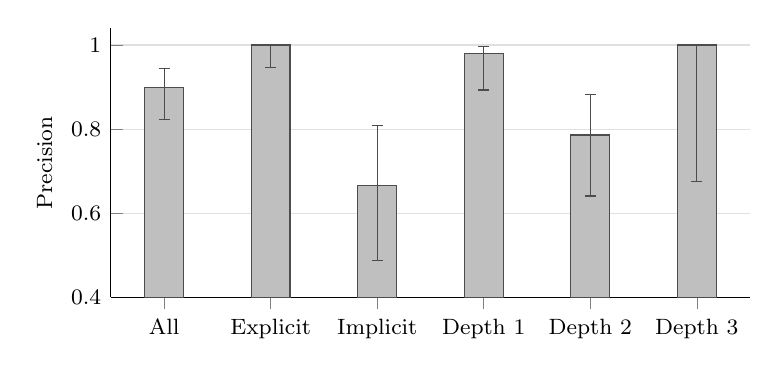
\begin{tikzpicture}
\begin{axis}[
  width=0.8\textwidth, height=5cm,
  ybar, bar width=14pt, ymin=0.4, ymax=1.04,
  ylabel={Precision}, ylabel style={font=\footnotesize},
  symbolic x coords={All,Explicit,Implicit,Depth 1,Depth 2,Depth 3},
  xtick=data, xticklabel style={font=\footnotesize},
  yticklabel style={font=\footnotesize},
  axis x line*=bottom, axis y line*=left,
  enlarge x limits=0.1, ymajorgrids, grid style={black!12},
  error bars/y dir=both, error bars/y explicit,
  error bars/error bar style={black!70}]
\addplot[fill=black!25, draw=black!70] coordinates {
  (All,0.899) += (0,0.045) -= (0,0.075)
  (Explicit,1.0) += (0,0) -= (0,0.053)
  (Implicit,0.667) += (0,0.141) -= (0,0.179)
  (Depth 1,0.98) += (0,0.016) -= (0,0.087)
  (Depth 2,0.786) += (0,0.097) -= (0,0.145)
  (Depth 3,1.0) += (0,0) -= (0,0.324)};
\end{axis}
\end{tikzpicture}
\caption{Precision of unreviewed links in the audit, with 95\% Wilson intervals}
\label{fig:precision}
\end{figure}

\paragraph{Error taxonomy.} Table~\ref{tab:errors} lists the ten links judged incorrect. All ten
rest on implied evidence at strength 1, and nine lie at depth 2. By relation, five are
\rel{escalates}, two \rel{motivates}, two \rel{prompts\_response} and one \rel{triggers}; the one
link judged unsure is also an implied \rel{escalates}. The auditor recorded a verdict but no reason,
so the categories below were assigned afterwards by reading each link's nodes and quotation:
\begin{itemize}
\item \emph{Continuity read as escalation} (5 links). Two links join two reports of the same
ongoing protest, opposition protests in Parliament over one issue during one session; the
quotation states that the protests continued, not that one caused the other. The other three join
two steps of one case or campaign (two arrests in one investigation, two phases of one political
march, a refusal and a later denial in one negotiation) that are related but not causally linked
as stated.
\item \emph{Quotation covers only one side} (2 links). The quotation describes the cause but not
the effect, so the text never states the link; in one case the second annotation had chosen a
different span that did describe the effect.
\item \emph{Reasoned rather than stated} (3 links). The link is plausible from background
knowledge but the quoted text does not state it: two links attribute a Supreme Court directive to
a farmer leader's hunger strike and his refusal of hospital care, and one treats an allotment
letter as the cause of the land dispute of which it is part.
\end{itemize}
The dominant failure is therefore not fabrication, which the verbatim check prevents, but
over-reading of implied evidence, chiefly within one campaign. A stricter re-annotation of the
implied links, tried as a filter, rejected 8 of the 10 wrong links but kept only 6 of the 20
correct ones, against a pre-set bar of 16, so it was not applied; the query service instead
withholds unreviewed implied links by default.

\begin{table}[!htbp]
\caption{The ten audited links judged incorrect. All rest on implied evidence. The last column is
the reason later given by the strict re-annotation, not by the human auditor, who recorded none.}
\label{tab:errors}
\footnotesize
\begin{tabularx}{\textwidth}{@{}lcXl@{}}
\toprule
Relation & Depth & Cause $\rightarrow$ effect (dates in 2024 unless stated) & Strict re-annotation \\
\midrule
\rel{escalates} & 2 & opposition protests in Parliament $\rightarrow$ INDIA bloc leaders protest (9 Dec, same day) & correlated only \\
\rel{escalates} & 2 & opposition parties protesting (28 Nov) $\rightarrow$ INDIA bloc MPs stage a protest (3 Dec) & duplicate event \\
\rel{escalates} & 2 & an arrest by the Enforcement Directorate (15 Mar) $\rightarrow$ a later arrest in the same case (7 Apr) & correlated only \\
\rel{escalates} & 2 & a political march sets off (Sep 2023) $\rightarrow$ its second phase (Jan) & insufficient evidence \\
\rel{escalates} & 2 & state rejects doctors' demand for a live broadcast (11 Sep) $\rightarrow$ state denies permission (14 Sep) & correlated only \\
\rel{prompts\_response} & 2 & activist announces a march on Mumbai (25 Feb) $\rightarrow$ Chief Minister warns him (26 Feb) & kept \\
\rel{prompts\_response} & 2 & farmer leader refuses hospitalisation $\rightarrow$ Supreme Court directive (28 Dec) & insufficient evidence \\
\rel{motivates} & 2 & farmer leader begins a fast unto death (26 Nov) $\rightarrow$ Supreme Court directs logistical support (28 Dec) & kept \\
\rel{motivates} & 1 & condition: payment still called an honorarium $\rightarrow$ anganwadi workers march (3 Jan) & insufficient evidence \\
\rel{triggers} & 2 & letter allotting university land (30 Nov) $\rightarrow$ condition: alienation of the land (from 3 Jun) & duplicate event \\
\bottomrule
\end{tabularx}
\end{table}

\subsection{Case studies}
\paragraph{Case 1: a three-link chain returned by a query.} Asked ``why were farmers protesting at the Punjab--Haryana border
in February 2024?'', Algorithm~\ref{alg:query} grounds the question in a story of 101 nodes and 185
links and returns, as its top chain, the demand for a legal minimum support price (MSP) guarantee,
which \rel{motivates} the \emph{Delhi Chalo} march (``began the `Delhi Chalo' march to Delhi on
February 13 to demand minimum support price for crops''), which \rel{prompts\_response} from
security forces who stop it at the border (``the police fired tear gas on the protestors''), which
\rel{triggers} the farmers' demonstration (``since February 13 after their march to Delhi was
stopped by security forces''). The next chain begins instead with the inconclusive talks of
12~February. Every link shown rests on explicit wording and links to its source article, and the
answer also lists 13 ancestors that were never searched. The march node itself folds in seven
duplicate records of the same event from other articles, and its \rel{motivates} link is supported by
four claims across seven outlets.

\paragraph{Case 2: from failed talks to a nationwide rail blockade.} A second chain through the
same node runs forward in time. The first round of talks with Union ministers on 8~February
\rel{escalates} into the last meeting on 12~February (implied evidence, confirmed by human
review: ``The first meeting with the Union ministers was held on February 8''); the
inconclusive outcome \rel{triggers} the march (``Farmers are heading towards Delhi after last
night's talks with Union ministers remained inconclusive''); the march \rel{escalates} into a
nationwide call issued on 3~March (``the two forums to spread this agitation countrywide call upon
the farmers and labourers across the country''); and that call \rel{mobilizes} the rail blockade
of 10~March (``they also gave a four-hour `rail roko' countrywide call for March 10 in support of
their demands''). The four quotations come from three outlets, and the chain spans a month, which no
single article reports.

\paragraph{Case 3: a failure.} An activist's announcement on 25~February that he would march on
Mumbai was linked by \rel{prompts\_response} to the Chief Minister's warning the next day. The
link is right in substance, but its quotation (``threatened to march to Mumbai to lay a siege at
his official residence'') describes only the cause, so the stored evidence does not state the link,
and the auditor rejected it. The second annotation had independently chosen a span that did describe
the response (``Chief Minister Eknath Shinde intervened and warned Jarange-Patil not to cross his
limits''). Because the gate requires only that the second annotation not reject a claim, it kept the
first annotation's quotation; requiring the stored quotation to mention both endpoints would have
caught this error, and is a cheap check to add.

\subsection{RQ4: querying and human effort}
The case study above shows that the graph answers causal questions with traceable chains. The
refusal rule was tested on adversarial questions: a question about a border between two places the
graph never links, or about a year other than 2024, is refused with the missing terms named, and
the closest story is offered instead. Questions whose words all occur in the graph but whose
meaning does not (for example, with actor roles swapped, negated or in the future tense) are not
caught by the rule; the list of matched words exposes them to the reader.

In the pilot a person issued 207 link verdicts for 176 published links, 1.18 per link. In the
scale-up no new human verdicts were made during construction (the pilot's verdicts stayed in $H$);
20{,}129 causal claims, 8{,}913 same-event pairs and 16{,}604 node pairs were annotated
automatically, and a person audited 100 links, 0.07 per published link. Human
verdicts per published link thus fell about seventeen-fold. Table~\ref{tab:guards} lists the errors
each safeguard caught before any person looked.

\begin{table}[!htbp]
\caption{Errors caught by each safeguard in the scale-up}
\label{tab:guards}
\footnotesize
\begin{tabular*}{\textwidth}{@{\extracolsep\fill}lr@{}}
\toprule
Safeguard & Caught \\
\midrule
Blind gate, main pass (links removed) & 143 \\
Blind gate, recovery rounds (links removed) & 32 \\
Cycle adjudication (links dropped) & 11 \\
Cannot-link constraint (merges blocked) & 5 \\
Re-annotation of merge decisions (merges reversed) & 4 \\
Date cap for undated stated causes (dates corrected) & 54 \\
Human audit (links removed) & 10 \\
\bottomrule
\end{tabular*}
\end{table}

\paragraph{Cost and duration.} Token usage, model calls and compute time were not logged, so we
report the measures that were recorded. Annotation ran as batches of claims handed to sub-agents, about 14 annotated claims per
retained link. No
paid API was used, and embeddings ran on a CPU. From screening of the 1{,}700 new articles to the
compiled graph took about three days of calendar time (11--14 November 2026). Human time was
about two hours for the pilot review of 207 links and about eight minutes for the 100-link audit.
Measuring tokens and wall-clock time per stage is left to future runs.

%% ---------------------------------------------------------------------------------------------
\section{Discussion and threats to validity}\label{sec:discussion}

The algorithm needs only GDELT-linked news text, a written rubric and an annotator, and nothing in
it is specific to protests. The evidence type recorded with every link proved the best predictor
of error, and exposing it costs nothing. Because causal claims about protests are politically
sensitive, the graph never states a link without its quotation and source, and declined candidates
are kept on record.

\subsection{Internal validity}
The first and second annotations were made by models of the same family. Their errors may be
correlated, and the gate would not catch an error both make; the pilot shows that the second
annotation never accepted a link the person rejected, but the pilot is small (207 links). Decoys
are earlier rejections, which may be easier to reject than the hardest wrong acceptances, so the
3\% decoy pass rate is a lower bound on permissiveness rather than an error rate. A later pass in
which one author accepted all 285 implied links in under three minutes is recorded as cursory and
excluded from every figure above.

\subsection{Construct validity}
The audit measures whether the quoted text supports the link as stated, not whether the cause is
true in the world. A correct link means that the source attributes the protest to the cause; the
graph is a structured record of reported causation, and its answers should be read that way.
Agreement $\kappa$ was measured between two independent annotations by the annotator, not between
two people.

\subsection{Conclusion validity}
Precision rests on one audit of 100 links by one person; the 95\% interval for overall precision
is 82--94\%, and the depth-3 interval is wide (8 links). Inter-rater agreement between people was
not measured, and about 900 explicit links remain unreviewed.

\subsection{External validity}
The study covers one country, one year, one event type and English-language reporting, and inherits
GDELT's source coverage. Recall is bounded by what the corpus reports: in the pilot, half of 103
causes documented by independent sources had no node, mostly because the corpus never reported
them. Screening and extraction labels were not reviewed by a person.

\subsection{Limitations and future work}
Some duplicate events remain, ongoing campaigns stay split by date, and expansion stops at three
levels. The query rule catches missing names, places and years but not swapped roles, negation or
tense. A campaign layer with a part-of relation would address the dominant error class directly, by
letting reports of one campaign be linked as parts of it rather than as escalations of each other;
review targeted at implied links, a second human auditor, and multilingual regional news are
natural next steps.

%% ---------------------------------------------------------------------------------------------
\section{Conclusion}\label{sec:conclusion}

GDELT records what happened; the articles behind it often say why. For RQ1, metadata alone
cannot separate causes from shuffled pairs. For RQ2, an independent second annotation calibrated
with decoys replaced per-link human review: in the pilot it never accepted a link a person
rejected, and at scale it passed 3\% of decoys. For RQ3, 90\% of unreviewed links were correct and
every link with explicit causal wording was, with errors concentrated in implied links between
reports of one ongoing protest. For RQ4, the graph answers causal questions with quoted, sourced
chains, refuses questions it cannot ground, and was built with about seventeen times fewer human
verdicts per link.

\backmatter

\bmhead{Acknowledgements}
Withheld for review.

\section*{Declarations}

\begin{itemize}
\item \textbf{Funding.} [To be completed by the authors.]
\item \textbf{Competing interests.} [To be completed by the authors.]
\item \textbf{Ethics approval.} Not applicable. The study uses published news articles and the
public GDELT event database; no human participants were involved apart from the authors' own
annotations.
\item \textbf{Data availability.} The compiled graph, rubrics, annotation records and measurement
reports are available in the anonymised repository [anonymised URL].
\item \textbf{Code availability.} The pipeline, compiler, query service and tests are available in
the anonymised repository [anonymised URL].
\item \textbf{Use of generative AI.} Large language model agents are part of the method and are
described in Section~\ref{sec:setup}. Separately, an AI assistant based on Claude helped write the
pipeline code and edit this manuscript under the authors' supervision. The authors verified every
reported figure and take responsibility for the content.
\end{itemize}

\bibliography{refs}

\end{document}
